% SYNTHETIC LAYOUT ONLY. No formal experiment outcomes are included.
\documentclass[letterpaper]{article}
\usepackage[T1]{fontenc}
\usepackage{spconf,amsmath,graphicx,booktabs}
\usepackage{newtxmath}
\usepackage[hidelinks]{hyperref}
\usepackage{eso-pic,xcolor}
\urlstyle{same}
\hypersetup{pdftitle={SYNTHETIC layout only - checkpoint-selection paper},pdfauthor={Tian Xie}}
\AddToShipoutPictureFG{\AtPageUpperLeft{\put(54,-20){\color{gray}\small SYNTHETIC LAYOUT ONLY - NOT RESEARCH RESULTS}}}
\newcommand{\slot}{\makebox[36pt]{---}}
\newcommand{\cislot}{\makebox[88pt]{[---, ---]}}
\title{Validation Speaker Exposure and Checkpoint Selection\\in Speech Emotion Recognition}
\name{Tian Xie}
\address{University of Toronto\\tianjack.xie@mail.utoronto.ca}
\begin{document}
\maketitle
\begin{abstract}
This is an explicitly synthetic page-budget sample, with no formal experimental results. The prospective paper examines familiar- versus unfamiliar-speaker checkpoint selection along a shared training trajectory and on an identical unfamiliar-speaker outer test. It compares cross-entropy and unweighted-average-recall criteria in three native speech-emotion tasks. The planned design contains 360 main trajectories and 24 fixed-last-epoch controls. Six prespecified tests use complete randomized draws, with separate descriptive analyses of absolute performance, full learning curves and training-group exchange. This space reserves the abstract's eventual quantitative findings and their limitations after complete execution and independent verification. It does not state a winning policy, a significant effect, equivalence, or a language mechanism. Its purpose is to verify that a full article can retain every planned outcome and the necessary interpretation within the conference page budget.
\end{abstract}
\begin{keywords}
speech emotion recognition, speaker independence, checkpoint selection, validation, evaluation
\end{keywords}
% Prospective framing only. No final-program outcomes have been read or inserted.
% Existing bibliography keys refer to english/main.tex and RELATED_WORK_AUDIT.md.
\section{Introduction}
Speech emotion recognition (SER) is often evaluated on speakers not used for training. Speaker separation is an established evaluation concern. SERAB and Antoniou et al. explicitly separate training, validation and test speakers~\cite{serab,antoniou}. More generally, optimizing a finite-sample selection criterion can affect subsequent performance evaluation~\cite{cawley}. However, a validation score difference and a difference in the selected models' performance on an identical unfamiliar-speaker test are distinct quantities. A larger validation--test gap alone does not establish that the corresponding selection rule produces a worse test model.

Prior SER studies already compare random and actor-independent evaluation across datasets, models or repeated runs~\cite{ibrahim,zielonka,kumari}; matching training counts across speaker/text conditions also has precedent~\cite{atmaja}. Such comparisons establish the relevance of evaluation protocols, but may change training or test membership along with the boundary of interest. We therefore study a specified checkpoint-selection comparison: validation on familiar versus unfamiliar speakers, each using either cross-entropy or unweighted average recall (UAR), along one shared training trajectory and on one shared speaker-exclusive outer test. Holding the candidate trajectory fixed removes differences between training runs from this within-trajectory comparison. The validation groups still contain different people, so the contrast concerns the complete selection policies rather than an isolated voiceprint mechanism.

This design follows earlier analyses of corpora already used in this project~\cite{artifact}. It fixes one model configuration, all 15 candidate epochs and the analysis before the new fits. The principal quantities are the common-test difference between the two cross-entropy policies and its interaction with the choice of cross-entropy versus UAR. All three native corpus tasks and all six planned tests are retained. Full trajectories and a fixed-last-epoch training-group exchange provide descriptive context; they do not supply additional hypothesis tests or determine which results are reported.


\section{Experimental design}
% Compact protocol alternative only: no new results or completion claim.
% C1--C8 correspond to final_program_methods_compact_zh.md.
\subsection{Shared-trajectory checkpoint-selection protocol}
\label{sec:final-program-methods}

% C1: Scope and prior exposure.
The protocol specifies 360 main trajectories: 24 draws and five outer folds
per corpus, plus 24 paired CREMA-D control fits. Checkpoint rules share a
training trajectory and speaker-independent outer test set. CREMA-D,
SUBESCO, and RAVDESS retain six, seven, and eight native classes and
91, 20, and 24 speakers, respectively~\cite{cremad,subesco,ravdess}.
These corpora have prior research exposure. The protocol uses a private
pre-execution source/plan freeze, not public preregistration. New draws do
not create previously untouched data.

% C2: Speaker/text allocation.
Within each draw, metadata hashing partitions speakers into five outer
folds, stratified by recorded sex; each speaker enters exactly one outer
fold. Outside each fold, disjoint development
groups A and B are sex-balanced and complete across chosen texts and
native classes. All query groups share texts disjoint from fit texts
(Table~\ref{tab:final-program-panels}); unused speakers remain excluded.
Frozen representatives are MD-preferred/otherwise XX for CREMA-D, T1 for
SUBESCO, and normal-intensity R1 for RAVDESS, without substitute takes.
Outer queries retain available representatives, requiring all native
classes for every outer speaker. Insufficient development capacity causes
metadata failure, not outcome-dependent resampling.

\begin{table}[t]
\centering
\caption{Prespecified per-context allocation. A and B are equal-sized,
sex-balanced groups; counts denote distinct speakers or recordings.}
\label{tab:final-program-panels}
\small
\setlength{\tabcolsep}{3pt}
\begin{tabular}{lrrrcrr}
\hline
Corpus & Classes & A/B & Outer & Texts$^a$ & Fit & Query$^b$\\
\hline
CREMA-D & 6 & 24/24 & 17/19 & 4/2 & 576 & 288\\
SUBESCO & 7 & 8/8 & 4 & 4/2 & 224 & 112\\
RAVDESS & 8 & 8/8 & 4/6 & 1/1 & 64 & 64\\
\hline
\end{tabular}
\par\raggedright\small
$^a$ Fit/query text counts. $^b$ Recordings in each of A and B query;
outer queries contain available CREMA-D representatives, 56 SUBESCO
recordings, or 32/48 RAVDESS recordings. Slash-separated outer counts
denote alternative fold sizes.
\end{table}

% C3: Fixed optimization.
Main trajectories train on A. WavLM base-plus~\cite{wavlm} has a
native-class linear head over mean-pooled final features; only the top
four Transformer layers and head are trainable. The earlier study's fixed
cfg3 uses AdamW,
encoder/head learning rates $5\times10^{-5}/10^{-3}$, weight decay 0.01,
batch size 16, and unweighted cross-entropy. All 15 epochs traverse the
fit set, without early stopping or hyperparameter search. Training uses
FP16 autocast with FP32 parameters; evaluation uses FP32.
Mono 16\,kHz audio is silence-trimmed at 30\,dB; training uses three-second crops
or zero-padding, and evaluation retains at most the first ten seconds.

% C4: Rules and padding context.
A queries provide seen-speaker validation; B queries provide unseen-speaker
validation. All 15 epochs record A, B, and outer logits. Four rules minimize
mean cross-entropy or maximize UAR on A or B; exact ties select the earliest
epoch, using rational recall to preserve exact UAR ties.
UAR is macro recall over native classes in the whole query group,
not average speaker UAR. Each group has separate sorted batches of 16,
fixed across epochs and paired models. Outer audio cannot pad validation
batches. Pooling lacks a length mask: padding context is fixed, but padding
effects remain.

\begin{table*}[t]
\centering\small
\caption{SYNTHETIC layout slots, not estimated values. The six common-test effects in UAR pp, pointwise 95\% draw-level $t$ intervals, and two-sided raw and six-family Holm $p$ values.}
\label{tab:primary}
\setlength{\tabcolsep}{5pt}
\begin{tabular}{llrrrr}\toprule
Corpus & Contrast & Mean & Pointwise 95\% CI & Raw $p$ & Holm $p$\\\midrule
CREMA-D & $\delta_{\mathrm{CE}}$ & \slot & \cislot & \slot & \slot\\
CREMA-D & $J$ & \slot & \cislot & \slot & \slot\\
SUBESCO & $\delta_{\mathrm{CE}}$ & \slot & \cislot & \slot & \slot\\
SUBESCO & $J$ & \slot & \cislot & \slot & \slot\\
RAVDESS & $\delta_{\mathrm{CE}}$ & \slot & \cislot & \slot & \slot\\
RAVDESS & $J$ & \slot & \cislot & \slot & \slot\\\bottomrule
\end{tabular}
\end{table*}

\begin{table*}[t]
\centering\small
\caption{SYNTHETIC layout slots only. Descriptive outer UAR (\%) of the four checkpoint policies and fixed epoch 15, plus $\delta_{\mathrm{UAR}}$ in pp; five folds then 24 draws are equally weighted.}
\label{tab:absolute}
\setlength{\tabcolsep}{5pt}
\begin{tabular}{lrrrrrr}\toprule
Corpus & Seen CE & Unseen CE & Seen UAR & Unseen UAR & Last 15 & $\delta_{\mathrm{UAR}}$\\\midrule
CREMA-D & \slot & \slot & \slot & \slot & \slot & \slot\\
SUBESCO & \slot & \slot & \slot & \slot & \slot & \slot\\
RAVDESS & \slot & \slot & \slot & \slot & \slot & \slot\\\bottomrule
\end{tabular}
\end{table*}

% C5: Estimands.
Let $T(g,q)$ be outer UAR in percent at the epoch selected by group
$g$ (seen $s$, unseen $u$) and criterion $q$. Per-context contrasts are
\begin{align}
\delta_q &= T(s,q)-T(u,q),\quad q\in\{\mathrm{CE},\mathrm{UAR}\},\\
J &= \delta_{\mathrm{CE}}-\delta_{\mathrm{UAR}}.
\end{align}
These are outer UAR differences in percentage points (pp), not loss or
validation-optimism ($V-T$) differences. They compare selection rules,
without identifying a unique speaker mechanism. Four rules reuse one
trajectory; they do not require four training runs.

% C6: Prespecified inference.
Within each corpus, five fold effects are averaged equally per draw.
Two-sided one-sample $t$ inference uses 24 complete draw effects ($df=23$).
The six-test family comprises $(\delta_{\mathrm{CE}},J)$ in three corpora,
with Holm control at 0.05 and pointwise 95\% $t$ intervals.
Undefined zero-variance tests remain NA, retaining their family slots.
Absolute UAR and $\delta_{\mathrm{UAR}}$ are descriptive. The 1\,pp practical
reference is not an equivalence margin; no equivalence test is performed.
Inference conditions on the finite corpus and training program; folds,
recordings, repeated speakers, and rules are not extra replicates.
Different native tasks preclude pooled inference or language-effect claims.

% C7: Paired group control.
CREMA-D fold 0 adds one B-trained model per draw, sharing initial weights,
matched stochastic schedules, and sex/text/class fit-slot budgets with A.
Within each sex, slots also match speaker rank, take, and intensity.
B trains for 15 epochs and records only final queries, without checkpoint
selection. For whole-group query UAR $Q_A,Q_B$ in percent,
\begin{equation}
\begin{aligned}
E=\tfrac12\{&[Q_A(M_{A,15})-Q_A(M_{B,15})]\\
&+[Q_B(M_{B,15})-Q_B(M_{A,15})]\}.
\end{aligned}
\end{equation}
The 24 pairs and their mean are descriptive. This replaces whole training
groups, not individual speakers; these queries also select main-A
checkpoints.

\begin{figure*}[t]
\centering
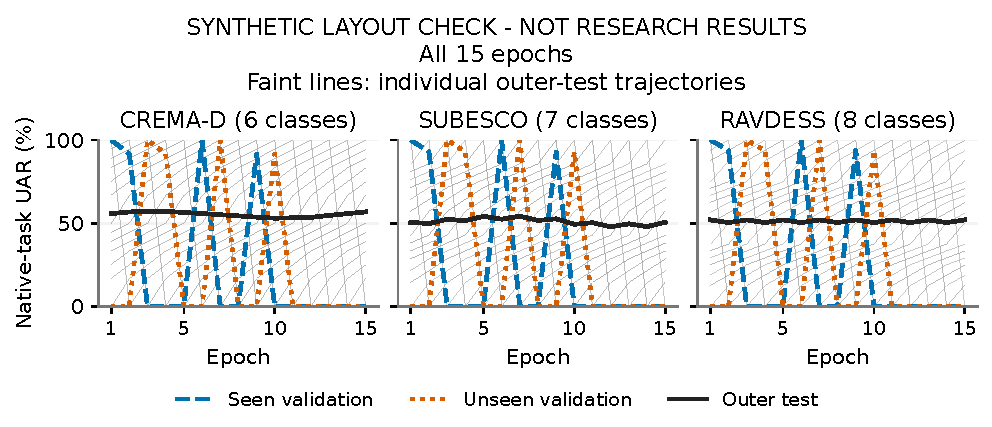
\includegraphics[width=178mm]{SYNTHETIC_curves.pdf}
\caption{SYNTHETIC LAYOUT ONLY. The final figure will retain all 15 epochs and all three native tasks. Faint grey lines are the 120 individual outer-test trajectories per corpus. The three heavy curves equally average the 120 main contexts for seen validation, unseen validation and outer testing. No smoothing or curve uncertainty bands are added.}
\label{fig:curves}
\end{figure*}

% C8: Sealing and diagnostics.
Four technical pilots are excluded from the 384 fits. Scoring requires
complete source, artifact, checkpoint, and ledger verification. Prespecified
descriptions retain selected-epoch distributions and agreement, all
15 epochs' outer curves, final UAR, epochs 8--10 minus 14--15 mean UAR,
and shortfall from each trajectory's maximum outer UAR. This oracle
neither selects retained checkpoints nor extends training. Full processing,
randomization, and verification details accompany the frozen protocol.

\section{Results: synthetic layout slots only}
\subsection{Prespecified common-test effects}
\textbf{No formal scores appear in this sample.} Table~\ref{tab:primary} reserves one row for each of the six prespecified tests. The final text will identify the direction, magnitude and uncertainty of both contrasts in each corpus, retaining disagreement and intervals crossing zero. The adjusted and unadjusted tests will be read from the accepted scoring output. Pointwise intervals will not be described as simultaneous intervals. Undefined tests will remain undefined rather than being converted to zero effects or favorable evidence. This paragraph also reserves room to distinguish statistical evidence from the one-percentage-point practical reference, and to explain precision where it limits an interpretation. No additional fitting, endpoint changes or result-dependent sample extension will follow inspection of these estimates.



\subsection{Absolute performance and selection behavior}
Table~\ref{tab:absolute} reserves all four selected-model outer UARs, the fixed last epoch and the descriptive UAR-rule contrast. This prevents a difference from obscuring the absolute performance of either policy. The final text will compare these quantities within each native task, without pooling class sets or attributing corpus differences to language. It will also report selected-epoch distributions, rule agreement, the descriptive outer-oracle shortfall, and the prespecified middle-minus-late-epoch descriptor. These summaries do not generate additional hypothesis tests or confidence intervals.





\subsection{Complete trajectories and whole-group exchange}
The synthetic curves in Fig.~\ref{fig:curves} verify only geometry. Final curve interpretation will describe the complete paths, including any plateaus, decline or disagreement, with selected-epoch summaries kept separate from the full trajectories. The CREMA-D exchange summary will retain all 24 fixed-last-epoch pairs and their mean. Its interpretation concerns replacement of an entire training group, with matched training slots and seeds. It does not isolate the causal contribution of a single speaker and does not turn queries used by the main selection rules into a globally untouched evaluation set.

\section{Discussion and relation to prior experiments}
This section reserves interpretation of the accepted common-test contrasts, including limitations on recommending any selection policy. The earlier N14R2 estimate concerns a change in validation optimism, $\Delta(V-T)$, under different inner procedures that also change fitting membership. It is not the same estimand as the present shared-trajectory outer-test comparison. DUAL and its subsequent diagnostics motivated this fixed-configuration, complete-trajectory study; the diagnostic analyses are post hoc uses of existing predictions rather than independent replication. The final account will keep these evidential roles distinct, rather than adding their effect estimates or increasing the inferential sample size by counting previous fits.

Related recording-budget and speaker-selection studies constrain the original data-construction question. With a fixed recording count, increasing speaker coverage also changes within-speaker text coverage. Improving a specified proxy for pool coverage does not by itself establish improved performance on unfamiliar speakers. The final report will retain these results and their specified models and budgets. The conditional synthetic-speech arm has not met its admission criteria; its technical generation attempts and incomplete human evaluation do not establish effective emotion- and identity-controlled augmentation.

\subsection{Scope of the comparison}
The estimates concern these finite acted-speech corpora and the specified randomization and training program. Repeated draws quantify variation within that program, not sampling of independent languages or corpora. The three tasks differ in their native classes, speaker counts, text coverage and training sizes; their differences cannot identify a language effect. Validation identities and recording distributions also differ between the familiar and unfamiliar groups. Fixing the trajectory therefore does not make speaker exposure an individually randomized causal intervention.

The training-group exchange changes an entire fit population. Its queries also participate in checkpoint selection for the main trajectories, although the exchange descriptor uses the fixed last epoch. It is not a separate globally unused blind test. Likewise, fixed report-group batches preserve padding context without removing the encoder's sensitivity to padding. Neither an interval crossing zero nor the absence of a significant adjusted test establishes equivalence; the 1-pp practical reference is not an equivalence margin tested by this program. Conclusions about which selection policy is preferable must follow the common-test estimates and their uncertainty, including any disagreement across corpora.

\subsection{Execution, evidence and availability}
This paragraph is reserved for the actual completed-unit count, failures or retries, source/plan binding, full artifact and ledger verification, independent numerical audit, and the predetermined fresh-process checkpoint-reload scope. It will report the observed coverage rather than reuse pilot counts. A portable prediction-evidence package will be distinguished from raw-audio retraining and full checkpoint verification. The research artifact is currently access-restricted; a private pre-execution freeze establishes a version history, not public preregistration. Original recordings, model bases and complete checkpoint evidence remain in their controlled archive. New formal results remain unavailable while training continues.

\section{Conclusion: reserved until full verification}
This synthetic document tests only layout. The eventual conclusion will answer the specified common-test question using every corpus and the complete prespecified family. It will state the strongest supported effect and the material uncertainty, distinguish model selection from validation optimism, and avoid promising that a dataset can eliminate the seen--unseen gap. No scientific verdict is supplied here.

\section{Acknowledgments and AI disclosure}
Anthropic Claude assisted original implementation, drafting and scientific review. OpenAI Codex assisted experiment design, implementation/execution, literature and analysis verification, and drafting/revision of all manuscript sections and tables. These systems are not authors; the named human author is responsible for reviewing the evidence and approving submission. The experiments use existing datasets; no new participant data were collected.

\clearpage
\begin{thebibliography}{12}
\raggedright
\bibitem{cawley} G. C. Cawley and N. L. C. Talbot, ``On over-fitting in model selection and subsequent selection bias in performance evaluation,'' \emph{Journal of Machine Learning Research}, vol. 11, no. 70, pp. 2079--2107, 2010.

\bibitem{atmaja} B. T. Atmaja and A. Sasou, ``Effect of different splitting criteria on the performance of speech emotion recognition,'' in \emph{Proc. TENCON}, 2021, pp. 760--764, doi: 10.1109/TENCON54134.2021.9707265.

\bibitem{antoniou} N. Antoniou, A. Katsamanis, T. Giannakopoulos, and S. Narayanan, ``Designing and evaluating speech emotion recognition systems: A reality check case study with IEMOCAP,'' in \emph{Proc. ICASSP}, 2023, pp. 1--5, doi: 10.1109/ICASSP49357.2023.10096808.

\bibitem{serab} N. Scheidwasser-Clow, M. Kegler, P. Beckmann, and M. Cernak, ``SERAB: A multi-lingual benchmark for speech emotion recognition,'' in \emph{Proc. ICASSP}, 2022, pp. 7697--7701, doi: 10.1109/ICASSP43922.2022.9747348.

\bibitem{zielonka} M. Zielonka et al., ``Recognition of emotions in speech using convolutional neural networks on different datasets,'' \emph{Electronics}, vol. 11, no. 22, Art. 3831, 2022, doi: 10.3390/electronics11223831.

\bibitem{ibrahim} E. Ibrahim, M. E. Ghoraba, and A. E. Ghoraba, ``Multimodal emotion recognition using hybrid deep feature fusion under speaker-independent evaluation,'' \emph{Scientific Reports}, vol. 16, Art. 19584, 2026, doi: 10.1038/s41598-026-58836-w.

\bibitem{kumari} P. Kumari et al., ``Hybrid CNN-embedding fusion with MFCC-SVM for speech emotion recognition: Random vs actor-wise evaluation on CREMA-D,'' \emph{PLOS One}, vol. 21, no. 8, Art. e0355238, 2026, doi: 10.1371/journal.pone.0355238.

\bibitem{artifact} T. Xie, ``SER experimental artifact: frozen v2 program and N14R2 corrective study,'' GitHub repository, 2026. [Online; access restricted at manuscript preparation]. \url{https://github.com/DeerNeverStop/SER}. Original historical tag: \texttt{SER26-prereg-1}; corrective-study historical tag: \texttt{SER26-N14R2-prereg-1}; completed analysis and erratum: \texttt{SER26-N14R2-complete-20260906}.

\bibitem{ravdess} S. R. Livingstone and F. A. Russo, ``The Ryerson Audio-Visual Database of Emotional Speech and Song (RAVDESS): A dynamic, multimodal set of facial and vocal expressions in North American English,'' \emph{PLOS ONE}, vol. 13, no. 5, Art. e0196391, 2018, doi: 10.1371/journal.pone.0196391.

\bibitem{cremad} H. Cao, D. G. Cooper, M. K. Keutmann, R. C. Gur, A. Nenkova, and R. Verma, ``CREMA-D: Crowd-sourced emotional multimodal actors dataset,'' \emph{IEEE Trans. Affective Computing}, vol. 5, no. 4, pp. 377--390, 2014, doi: 10.1109/TAFFC.2014.2336244.

\bibitem{subesco} S. Sultana, M. S. Rahman, M. R. Selim, and M. Z. Iqbal, ``SUST Bangla Emotional Speech Corpus (SUBESCO): An audio-only emotional speech corpus for Bangla,'' \emph{PLOS ONE}, vol. 16, no. 4, Art. e0250173, 2021, doi: 10.1371/journal.pone.0250173.

\bibitem{wavlm} S. Chen et al., ``WavLM: Large-scale self-supervised pre-training for full stack speech processing,'' \emph{IEEE J. Sel. Topics Signal Process.}, vol. 16, no. 6, pp. 1505--1518, 2022, doi: 10.1109/JSTSP.2022.3188113.

\end{thebibliography}
\end{document}
